\documentclass{standalone}
\usepackage{tikz}
\usetikzlibrary{patterns, positioning}


\begin{document}
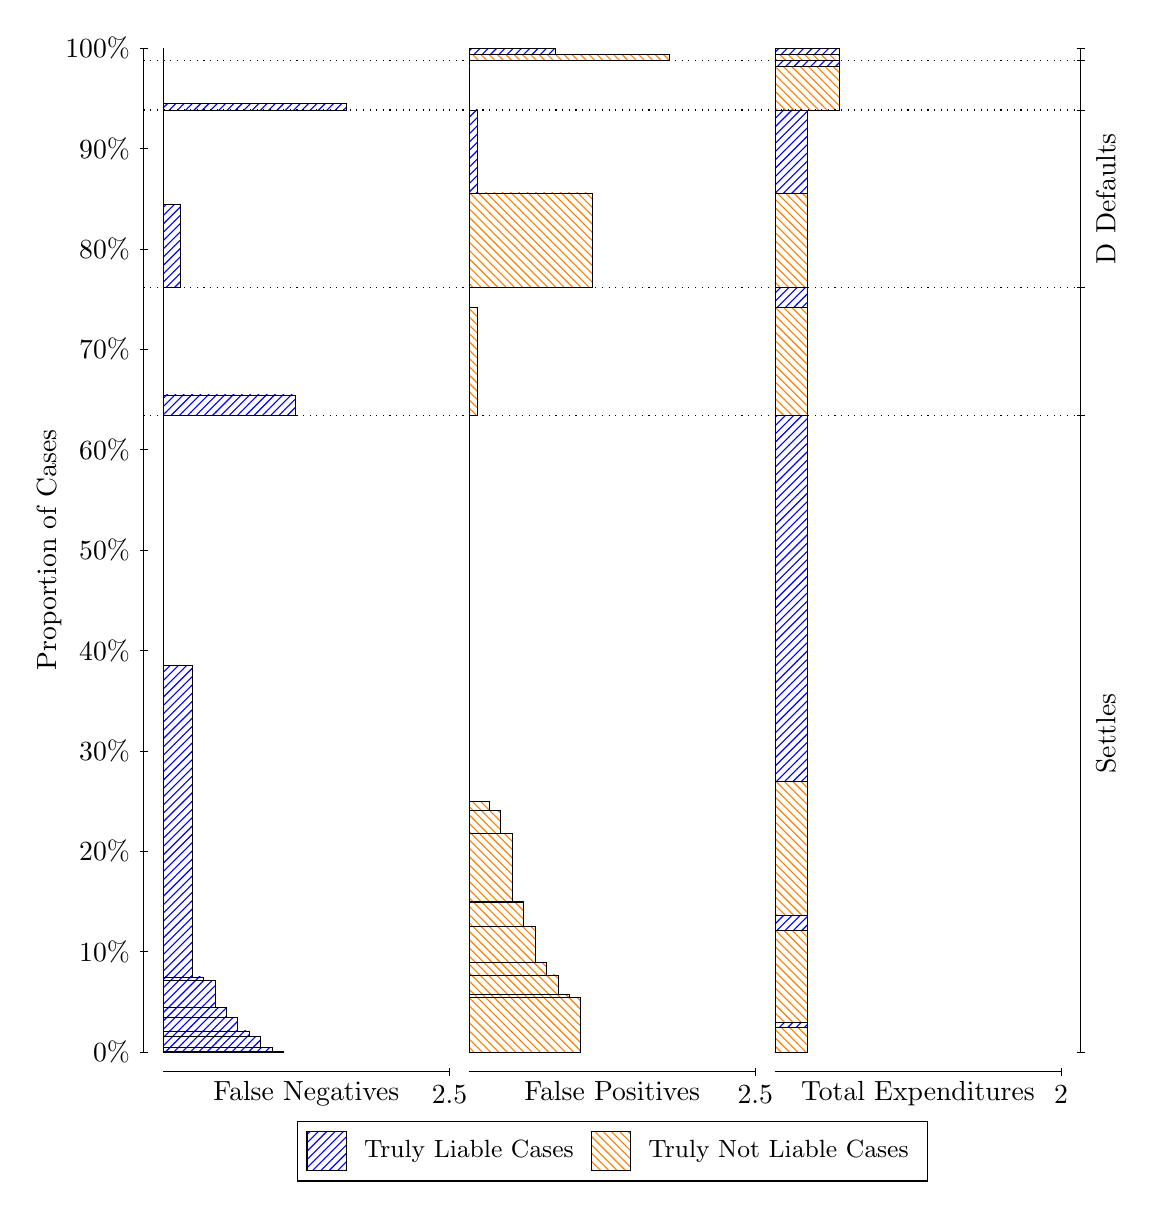
\begin{tikzpicture}
\draw[black, very thin] (1.5,1.75) -- (1.5,14.5);
\node[rotate=90, text=black, anchor=center] at (0.3, 8.125) {Proportion of Cases};
\draw[black, very thin] (1.45,1.75) -- (1.55,1.75);
\node[text=black, anchor=east] at (1.45, 1.75) {0\%};
\draw[black, very thin] (1.45,3.025) -- (1.55,3.025);
\node[text=black, anchor=east] at (1.45, 3.025) {10\%};
\draw[black, very thin] (1.45,4.3) -- (1.55,4.3);
\node[text=black, anchor=east] at (1.45, 4.3) {20\%};
\draw[black, very thin] (1.45,5.575) -- (1.55,5.575);
\node[text=black, anchor=east] at (1.45, 5.575) {30\%};
\draw[black, very thin] (1.45,6.85) -- (1.55,6.85);
\node[text=black, anchor=east] at (1.45, 6.85) {40\%};
\draw[black, very thin] (1.45,8.125) -- (1.55,8.125);
\node[text=black, anchor=east] at (1.45, 8.125) {50\%};
\draw[black, very thin] (1.45,9.4) -- (1.55,9.4);
\node[text=black, anchor=east] at (1.45, 9.4) {60\%};
\draw[black, very thin] (1.45,10.675) -- (1.55,10.675);
\node[text=black, anchor=east] at (1.45, 10.675) {70\%};
\draw[black, very thin] (1.45,11.95) -- (1.55,11.95);
\node[text=black, anchor=east] at (1.45, 11.95) {80\%};
\draw[black, very thin] (1.45,13.225) -- (1.55,13.225);
\node[text=black, anchor=east] at (1.45, 13.225) {90\%};
\draw[black, very thin] (1.45,14.5) -- (1.55,14.5);
\node[text=black, anchor=east] at (1.45, 14.5) {100\%};

\draw[black, very thin] (13.4,1.75) -- (13.4,14.5);
\draw[black, very thin] (13.35,1.75) -- (13.45,1.75);
\node[anchor=west] at (13.35, 1.75) {};
\draw[black, very thin] (13.35,9.8388) -- (13.45,9.8388);
\node[anchor=west] at (13.35, 9.8388) {};
\draw[black, very thin] (13.35,11.463) -- (13.45,11.463);
\node[anchor=west] at (13.35, 11.463) {};
\draw[black, very thin] (13.35,13.713) -- (13.45,13.713);
\node[anchor=west] at (13.35, 13.713) {};
\draw[black, very thin] (13.35,14.343) -- (13.45,14.343);
\node[anchor=west] at (13.35, 14.343) {};
\draw[black, very thin] (13.35,14.5) -- (13.45,14.5);
\node[anchor=west] at (13.35, 14.5) {};

\draw[black, very thin, pattern color=blue, pattern=north east lines] (1.75,1.75) rectangle (3.276,1.7601);
\draw[black, very thin, pattern color=blue, pattern=north east lines] (1.75,1.7601) rectangle (3.1307,1.8046);
\draw[black, very thin, pattern color=blue, pattern=north east lines] (1.75,1.8046) rectangle (2.9853,1.9479);
\draw[black, very thin, pattern color=blue, pattern=north east lines] (1.75,1.9479) rectangle (2.84,2.0165);
\draw[black, very thin, pattern color=blue, pattern=north east lines] (1.75,2.0165) rectangle (2.6947,2.1876);
\draw[black, very thin, pattern color=blue, pattern=north east lines] (1.75,2.1876) rectangle (2.5493,2.3134);
\draw[black, very thin, pattern color=blue, pattern=north east lines] (1.75,2.3134) rectangle (2.404,2.6547);
\draw[black, very thin, pattern color=blue, pattern=north east lines] (1.75,2.6547) rectangle (2.2587,2.7049);
\draw[black, very thin, pattern color=blue, pattern=north east lines] (1.75,2.7049) rectangle (2.1133,6.6551);
\draw[black, very thin, pattern color=orange, pattern=north west lines] (1.75,6.6551) rectangle (1.75,9.8388);
\draw[black, very thin, pattern color=blue, pattern=north east lines] (1.75,9.8388) rectangle (3.4213,10.095);
\draw[black, very thin, pattern color=orange, pattern=north west lines] (1.75,10.095) rectangle (1.75,11.463);
\draw[black, very thin, pattern color=blue, pattern=north east lines] (1.75,11.463) rectangle (1.968,12.518);
\draw[black, very thin, pattern color=orange, pattern=north west lines] (1.75,12.518) rectangle (1.75,13.713);
\draw[black, very thin, pattern color=blue, pattern=north east lines] (1.75,13.713) rectangle (4.0753,13.794);
\draw[black, very thin, pattern color=orange, pattern=north west lines] (1.75,13.794) rectangle (1.75,14.343);
\draw[black, very thin, pattern color=orange, pattern=north west lines] (1.75,14.343) rectangle (1.75,14.421);
\draw[black, very thin, pattern color=blue, pattern=north east lines] (1.75,14.421) rectangle (1.75,14.5);
\draw[black, very thin, pattern color=orange, pattern=north west lines] (5.6333,1.75) rectangle (7.0503,2.4402);
\draw[black, very thin, pattern color=orange, pattern=north west lines] (5.6333,2.4402) rectangle (6.905,2.4851);
\draw[black, very thin, pattern color=orange, pattern=north west lines] (5.6333,2.4851) rectangle (6.7597,2.7294);
\draw[black, very thin, pattern color=orange, pattern=north west lines] (5.6333,2.7294) rectangle (6.6143,2.8903);
\draw[black, very thin, pattern color=orange, pattern=north west lines] (5.6333,2.8903) rectangle (6.469,3.344);
\draw[black, very thin, pattern color=orange, pattern=north west lines] (5.6333,3.344) rectangle (6.3237,3.6558);
\draw[black, very thin, pattern color=orange, pattern=north west lines] (5.6333,3.6558) rectangle (6.3237,3.6586);
\draw[black, very thin, pattern color=orange, pattern=north west lines] (5.6333,3.6586) rectangle (6.1783,4.5276);
\draw[black, very thin, pattern color=orange, pattern=north west lines] (5.6333,4.5276) rectangle (6.033,4.8197);
\draw[black, very thin, pattern color=orange, pattern=north west lines] (5.6333,4.8197) rectangle (5.8877,4.9336);
\draw[black, very thin, pattern color=blue, pattern=north east lines] (5.6333,4.9336) rectangle (5.6333,9.8388);
\draw[black, very thin, pattern color=orange, pattern=north west lines] (5.6333,9.8388) rectangle (5.7423,11.207);
\draw[black, very thin, pattern color=blue, pattern=north east lines] (5.6333,11.207) rectangle (5.6333,11.463);
\draw[black, very thin, pattern color=orange, pattern=north west lines] (5.6333,11.463) rectangle (7.1957,12.659);
\draw[black, very thin, pattern color=blue, pattern=north east lines] (5.6333,12.659) rectangle (5.7423,13.713);
\draw[black, very thin, pattern color=orange, pattern=north west lines] (5.6333,13.713) rectangle (5.6333,14.263);
\draw[black, very thin, pattern color=blue, pattern=north east lines] (5.6333,14.263) rectangle (5.6333,14.343);
\draw[black, very thin, pattern color=orange, pattern=north west lines] (5.6333,14.343) rectangle (8.1767,14.421);
\draw[black, very thin, pattern color=blue, pattern=north east lines] (5.6333,14.421) rectangle (6.7233,14.5);
\draw[black, very thin, pattern color=orange, pattern=north west lines] (9.5167,1.75) rectangle (9.9254,2.0618);
\draw[black, very thin, pattern color=blue, pattern=north east lines] (9.5167,2.0618) rectangle (9.9254,2.1296);
\draw[black, very thin, pattern color=orange, pattern=north west lines] (9.5167,2.1296) rectangle (9.9254,3.2935);
\draw[black, very thin, pattern color=blue, pattern=north east lines] (9.5167,3.2935) rectangle (9.9254,3.4821);
\draw[black, very thin, pattern color=orange, pattern=north west lines] (9.5167,3.4821) rectangle (9.9254,5.19);
\draw[black, very thin, pattern color=blue, pattern=north east lines] (9.5167,5.19) rectangle (9.9254,9.8388);
\draw[black, very thin, pattern color=orange, pattern=north west lines] (9.5167,9.8388) rectangle (9.9254,11.207);
\draw[black, very thin, pattern color=blue, pattern=north east lines] (9.5167,11.207) rectangle (9.9254,11.463);
\draw[black, very thin, pattern color=orange, pattern=north west lines] (9.5167,11.463) rectangle (9.9254,12.659);
\draw[black, very thin, pattern color=blue, pattern=north east lines] (9.5167,12.659) rectangle (9.9254,13.713);
\draw[black, very thin, pattern color=orange, pattern=north west lines] (9.5167,13.713) rectangle (10.334,14.263);
\draw[black, very thin, pattern color=blue, pattern=north east lines] (9.5167,14.263) rectangle (10.334,14.343);
\draw[black, very thin, pattern color=orange, pattern=north west lines] (9.5167,14.343) rectangle (10.334,14.421);
\draw[black, very thin, pattern color=blue, pattern=north east lines] (9.5167,14.421) rectangle (10.334,14.5);
\draw[black, dotted] (1.5,9.8388) -- (13.4,9.8388);
\draw[black, dotted] (1.5,11.463) -- (13.4,11.463);
\draw[black, dotted] (1.5,13.713) -- (13.4,13.713);
\draw[black, dotted] (1.5,14.343) -- (13.4,14.343);
\draw[black, very thin] (1.75,1.5) -- (5.3833,1.5);
\node[text=black, anchor=north] at (3.5667, 1.5) {False Negatives};
\draw[black, very thin] (5.3833,1.45) -- (5.3833,1.55);
\node[text=black, anchor=north] at (5.3833, 1.45) {2.5};

\draw[black, very thin] (5.6333,1.5) -- (9.2667,1.5);
\node[text=black, anchor=north] at (7.45, 1.5) {False Positives};
\draw[black, very thin] (9.2667,1.45) -- (9.2667,1.55);
\node[text=black, anchor=north] at (9.2667, 1.45) {2.5};

\draw[black, very thin] (9.5167,1.5) -- (13.15,1.5);
\node[text=black, anchor=north] at (11.333, 1.5) {Total Expenditures};
\draw[black, very thin] (13.15,1.45) -- (13.15,1.55);
\node[text=black, anchor=north] at (13.15, 1.45) {2};

\node[text=black, centered, rotate=90] at (13.72, 5.7944) {Settles};

\node[text=black, centered, rotate=90] at (13.72, 12.588) {D Defaults};



\draw (7.449999999999999,1.5) node[draw=none] (baseCoordinate) {};
\begin{scope}[align=center]
        \matrix[scale=0.5, draw=black, below=0.5cm of baseCoordinate, nodes={draw}, column sep=0.1cm]{
            \node[rectangle, draw, minimum width=0.5cm, minimum height=0.5cm, pattern color=blue, pattern=north east lines] {}; &
            \node[draw=none, font=\small, text=black] (B) {Truly Liable Cases}; &
            \node[rectangle, draw, minimum width=0.5cm, minimum height=0.5cm, pattern color=orange, pattern=north west lines] {}; &
            \node[draw=none, font=\small, text=black] (B) {Truly Not Liable Cases}; \\
            };
\end{scope}

\end{tikzpicture}
\end{document}